\subsection{Data Pipeline}\label{sec:data-pipeline}
Two datasets are used in this thesis. The first is the TTF futures dataset, which is used to train and evaluate the model. The second is the TTF options dataset, which provides the market prices for the benchmark in Sec.~\ref{sec:pricing-setup}.

\subsubsection{Futures Data}\label{sec:futures-data}
The futures data was obtained from BASF's Bloomberg infrastructure and covers
TTF natural gas futures for the first three nearby contracts between January
2010 and April 2026. The data is distributed as three schemas: contract prices, contract metadata, and monthly listings of active contracts.

\textbf{Daily settlement prices.} This schema provides the price history of the contracts in the dataset.  Each contract is observed once per trading day, identified by contract symbol and trading date. Each record contains opening, high, low and daily closing prices in EUR/MWh, trading volume and open interest. Coverage of these fields varies considerably with how actively a contract was traded and how far from expiry it is. The closing price is the exception and is available throughout the whole dataset. Additionally, it falls outside the intraday high–low range for \num{7712} of \num{25884}  records, or \SI{29.8}{\percent}. The deviation is small in most cases, with a median of \num{0.10} EUR/MWh, but reaches up to \num{42.26} EUR/MWh. The latter confirms that it is a settlement price set by the exchange rather than a price at which trading occurred.

\textbf{Contract metadata.} This schema provides static attributes per unique contract in the dataset. The expiry date provided per record is used to rank contracts by time to maturity in Sec.~\ref{sec:m1-construction}. All contracts in the dataset are physically delivered instruments traded on ICE Endex and quoted in EUR/MWh. First and last trading dates, notice dates and delivery dates are also recorded.

\textbf{Contract listings.} This schema records which contracts were active on the market, as monthly snapshots taken on the first calendar day of each month. Each contract is observed once per snapshot. Together with the expiry dates, the listings determine which contract is the front month on a given date, as described in Sec.~\ref{sec:m1-construction}.

\subsubsection{Front-Month Series Construction}\label{sec:m1-construction}
As described in Sec.~\ref{sec:futures-data}, the contract listings and the
contract metadata each hold part of the information required to identify
the front-month contract. The listings record which contracts were active in a
given month, while the metadata records when each contract expires. Therefore, the expiry dates were joined onto the listings by contract symbol. As a result, each listing record carries the expiry date of the contract it refers to. 

The contracts were then sorted by expiry date within each monthly snapshot and the earliest-expiring one was kept. This gives the front-month contract for that month. Since the snapshots are monthly, but the series must be daily, each trading day was assigned the front-month contract from the most recent snapshot on or before that day.
The settlement price of the selected contract was then added for each trading day, matching on trading date and contract symbol. The trading days without an available settlement price were discarded. The resulting series contains \num{3998} trading days spanning 2010-01-04 to 2026-04-24, with settlement prices ranging from \num{3.509} to \num{339.196}~EUR/MWh. The construction of the front-month series is implemented in \texttt{build\_front\_month.py}.

Since the front-month contract is replaced at each expiry, the series is not the price history of a single instrument. The listings are monthly snapshots, so the front-month contract switches on the first trading day of each month. The days between the last trading day of the contract and the next listing do not carry a settlement price. These days were discarded from the series.\footnote{Trading in a TTF futures
contract ceases two UK business days before the first day of the delivery month.} Returns spanning a contract transition cover two to six calendar days, with a median of four, and reflect the change in the price level as well as the difference between the two contracts. Across the \num{195} transition days in the sample, the standard deviation of log returns is \num{0.071}, compared to \num{0.037} on all other days. When the transition days are excluded, excess kurtosis falls from \num{14.91} to \num{14.65}, and skewness from \num{0.70} to \num{0.26}.\footnote{Skewness and excess kurtosis are computed with the sample estimators $g_1$ and $g_2$ of Eq.~\eqref{eq:g1-g2}.} Transition days contribute little to the tail weight of the series, but they are responsible for most of its positive skew. 


The transition effect described above is preserved and quantified rather than removed, since restricting the analysis to a single contract would reduce the sample to a few months.

\subsubsection{Return Definition}\label{sec:return-definition}
The original Fin-GAN input series is built from two returns per day \parencite{vuleticFinGANForecastingClassifying2024}. The first is the intraday return, from the opening to the closing price and the second is the overnight return, from one closing price to the next opening
price. The return of the corresponding sector ETF is then subtracted from each entry. This isolates the part of the movement specific to the asset.

Neither step has been adopted for the TTF futures dataset. The two-return scheme requires opening and closing prices that are both traded prices. As shown in Sec.~\ref{sec:futures-data}, the daily price in this dataset is a settlement price set by the exchange. A return computed between the opening trade and the settlement price would therefore combine two different price concepts.

Additionally, the excess-return step requires a benchmark that leaves a meaningful residual when subtracted. In the case of equities, subtracting the sector ETF return removes the market-wide component and leaves the movement specific to the individual stock. European natural gas has no comparable instrument.

As a substitute, the second nearby contract was considered. However, the difference between the first and second nearby returns is a calendar spread return, as described in Sec.~\ref{sec:futures}. A model that is trained on it would learn how the gap between two contracts moves, not how the gas price itself moves. Option payoffs depend on the price level at expiry, so a model trained on spread returns could not be used to price options.

Therefore, the dataset was constructed from daily logarithmic returns of the front-month settlement price. Returns are approximately stationary and therefore comparable across the sample period. Additionally, log returns are additive across time and allow price levels to be recovered exactly from simulated returns. The latter is required for the Monte Carlo procedure
in Sec.~\ref{sec:pricing-setup}.

\begin{equation}\label{eq:logreturn}
    x_t = \log\!\left(\frac{P_t}{P_{t-1}}\right),
\end{equation}
where $P_t$ is the front-month settlement price on trading day $t$.
The transformation gives \num{3997} return observations.

\subsubsection{Data Split}\label{sec:data-split}
The return series was split chronologically into training (\SI{80}{\percent}), validation (\SI{10}{\percent}), and test (\SI{10}{\percent}) sets using the proportions of \textcite{vuleticFinGANForecastingClassifying2024}. Training covers 2010-01-05 to 2023-01-18
validation 2023-01-19 to 2024-09-04 (\num{399} returns), and test
2024-09-05 to 2026-04-24 (\num{401} returns).
\begin{figure}[htbp]
    \centering
    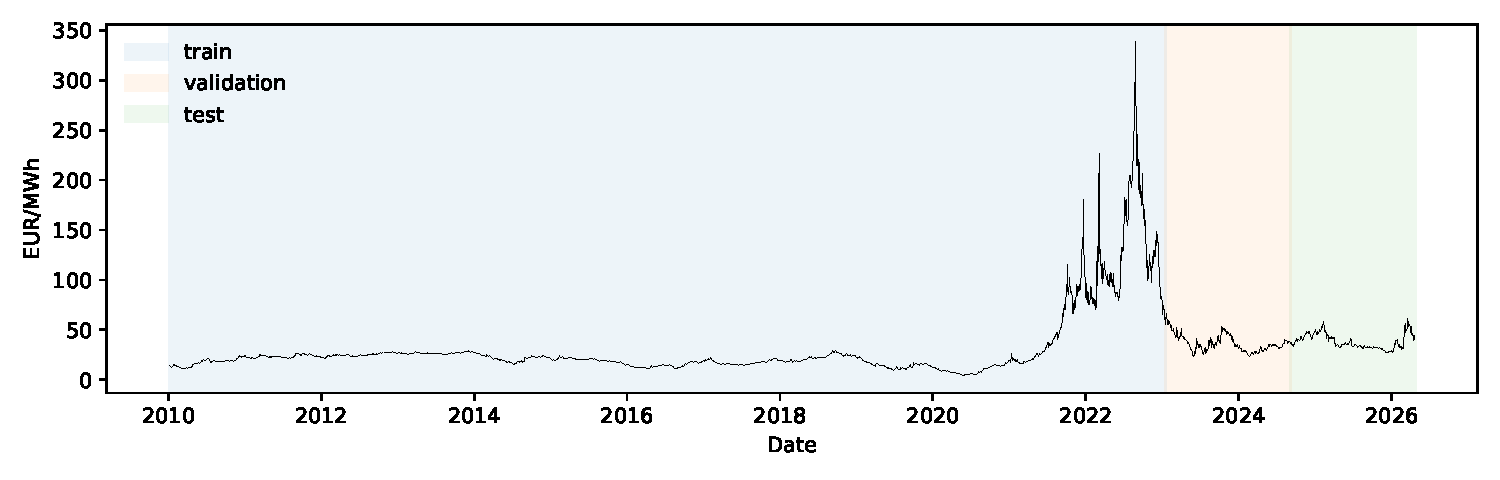
\includegraphics[width=\textwidth]{figures/ttf_price_split.pdf}
    \caption{TTF train, validation and test data split}
    \label{fig:ttf-price-split}
\end{figure}

The chronological split was explicitly used to avoid look-ahead bias. Following the current split, the 2021 to 2022 price disruption discussed in Sec.~\ref{sec:gas-markets} falls entirely within the training period, and the 2026 disruption falls entirely within the test period, as seen in Fig.~\ref{fig:ttf-price-split}.

Sliding window matrices were constructed for each split separately, so that no window spans a split boundary. The window was moved forward by one trading day.

\subsubsection{Options Data}\label{sec:options-data}

The TTF options data was obtained from Databento and covers ICE Endex TTF natural gas options. Contract records span March 2019 to June 2026, and daily settlement prices are available from March 2023 to June 2026. The price coverage contains the full test split of Sec.~\ref{sec:data-split}. The data is distributed as five schemas: Definition, Statistics, Best bid and offer (BBO), Open High Low Close Volume (OHLCV), and Status. 

\textbf{Definition.} Contract metadata is provided per instrument in the dataset. All options are European and quoted in EUR/MWh, matching the futures dataset of Sec.~\ref{sec:futures-data}. The underlying of each option is a front-month TTF futures contract. Instrument classes present in the dataset are calls, puts, calendar spread instruments and multi-leg instruments. Calendar spread instruments hold a long position in one delivery month and a short position in another. Their value depends on the calendar spread of Sec.~\ref{sec:futures} rather than on the price level. Multi-leg instruments combine multiple options into a single contract. Neither class has a strike price, so the payoff described in Sec.~\ref{sec:options} is undefined for them. Only call and put options were kept. This leaves \num{15005854} of the \num{56882528} records in the schema, split evenly between calls and puts. Strike prices range from \num{0.50} to \num{1000} EUR/MWh across \num{510} distinct values, and contracts carry \num{142} distinct expiry dates, one per calendar month. This schema is an event log, where each record describes a change in the metadata of a contract. The most recent record for each contract was retained, giving \num{35952} contracts.

\textbf{Statistics.} Daily statistics are provided per statistic, contract and trading day. The schema holds \num{99307437} records, of which \num{60664334} are put and call options. It contains settlement prices and implied volatilities, alongside further statistics that are not used, leaving \num{17424688} records. The implied volatility is published by the exchange, so the numerical procedure of Sec.~\ref{sec:implied-vol} is not required for the market prices. The dataset contains final and preliminary records, of which only the final ones are kept. \num{5807828} records are retained for settlement prices and \num{5812246} for implied volatilities. \num{392904} contract-days carry a duplicate record, of which \num{4128}, around \SI{1}{\percent}, carry a different price. These cluster on a few dates and are consistent with revisions published by the exchange. To ensure that revised prices are used, the record with the highest sequence number was retained. The resulting panel contains \num{11231588} records for \num{20252} contracts, around \SI{56}{\percent} of the \num{35952} contracts in the dataset.

\textbf{BBO.} The schema records the best bid and ask prices in a sequence of snapshots through each trading day. A bid and an ask together are referred to as a quote. The quote is two-sided when both are present. The schema covers the period from 2023-05-02 to 2026-06-26. However, two-sided quotes are almost absent at the start of that period, with \num{2485} in 2023 and \num{2069} in 2024 against \num{25969129} in 2025. The test split of Sec.~\ref{sec:data-split} begins on 2024-09-05, so the quotes would cover only part of it. 

\textbf{OHLCV.} The schema records the opening, high, low and closing prices, together with the trading volume, in one-minute bars. The schema covers 2023-03-20 to 2026-06-26. Each bar summarizes the trades in a single contract over one minute. Of the \num{365892} bars, \num{340313} are on-exchange and the remainder are off-market trades that print at different prices. Only \num{4327} of the \num{20252} contracts with settlement prices have any trades, around \SI{21}{\percent}. Out of all the days when an option received an official settlement price, only \SI{0.47}{\percent} also had a trade. As a result, the schema does not provide a continuous price series. 

\textbf{Status.} The schema records whether each contract was open for trading and whether it was open for quoting. The schema does not provide price information and is not used in this thesis.

The contract definitions and daily statistics each hold part of the information required. The definitions hold the strike price and the expiry date, while the statistics hold the settlement price and the implied volatility. The two schemas were joined by contract identifier. The front-month series of Sec.~\ref{sec:m1-construction} was then joined by the trading date to provide the front-month settlement price and the moneyness defined in Sec.~\ref{sec:options} for each option. The moneyness of an option is exact only when the underlying is the front-month contract, since the series carries the price of whichever contract is front month on that date. This holds close to expiry. Each row of the panel is one contract on one trading day, and also carries the number of days from the trading date to expiry. In total there are \num{5615794} records for \num{20252} contracts. The days between the last trading day of a contract and the next front-month listing do not carry a front-month settlement price, so \num{268598} records have no moneyness. A further \num{181950} records fall after 2026-04-24, the end of the futures series, and also do not carry moneyness. The construction of the options panel is implemented in \texttt{build\_options\_panel.py}.

The panel spans March 2023 to June 2026, while the test split of Sec.~\ref{sec:data-split} covers September 2024 to April 2026. It was restricted to the test split, resulting in \num{1763210} records for \num{9144} contracts. Three groups of records were then filtered out. \num{5062} records on the expiry date have a time to maturity of zero, so no pricing method applies to them. A further \num{81584} records fall on the days without a front-month settlement price, described above. Lastly, a moneyness band of \num{0.5} to \num{2.0} was applied. Since the median settlement price falls smoothly with moneyness, there is no natural break in the data, so the bounds were set as follows. Below the \num{0.5} lower bound, the implied volatility rises and becomes erratic. Almost all the option value is the amount it would pay if exercised immediately, and the volatility is recovered from the small remainder. Above the \num{2.0} upper bound, the median settlement price approaches the exchange minimum tick of \num{0.005}, so the price does not carry information. The resulting panel contains \num{1250980} records for \num{7208} contracts. The filtering of the options panel is implemented in \texttt{filter\_options\_panel.py}.